\documentclass[10pt,twocolumn,letterpaper]{article}

\usepackage{3dv}
\usepackage{times}
\usepackage{epsfig}
\usepackage{graphicx}
\usepackage{amsmath}
\usepackage{amssymb}

% added packages
\usepackage{subcaption}
\usepackage{multirow}
\usepackage{array}
\usepackage{slashbox}
% Include other packages here, before hyperref.

% If you comment hyperref and then uncomment it, you should delete
% egpaper.aux before re-running latex.  (Or just hit 'q' on the first latex
% run, let it finish, and you should be clear).
\usepackage[pagebackref=true,breaklinks=true,letterpaper=true,colorlinks,bookmarks=false]{hyperref}


%\threedvfinalcopy % *** Uncomment this line for the final submission

\def\threedvPaperID{****} % *** Enter the 3DV Paper ID here
\def\httilde{\mbox{\tt\raisebox{-.5ex}{\symbol{126}}}}

% Pages are numbered in submission mode, and unnumbered in camera-ready
\ifthreedvfinal\pagestyle{empty}\fi
\begin{document}

%%%%%%%%% TITLE
\title{Recurrent Neural Network based Sign Language Recognition using 3D Skeleton Data}

\author{First Author\\
Institution1\\
Institution1 address\\
{\tt\small firstauthor@i1.org}
% For a paper whose authors are all at the same institution,
% omit the following lines up until the closing ``}''.
% Additional authors and addresses can be added with ``\and'',
% just like the second author.
% To save space, use either the email address or home page, not both
\and
Second Author\\
Institution2\\
First line of institution2 address\\
{\tt\small secondauthor@i2.org}
}

\maketitle
% \thispagestyle{empty}

%%%%%%%%% ABSTRACT
\begin{abstract}
Video based sign language recognition is a mature problem in the computer vision community. With the recent upsurge of depth sensor, 3D video data -- RGB with depth information -- has become a popular choice for video analysis because of its extra depth modality. Another type of 3D data -- 3D skeleton data -- has shown extensive usage in human activity understanding and become part of state-of-art methods in this domain. Despite having similarity with the human activity recognition, use of 3D skeleton data in sign language recognition is scarce. One of the few reasons behind this is unavailability of a benchmark public dataset. In this paper, we introduce a 3D skeleton dataset for American sign language (ASL) recognition. The dataset has RGB, depth, skeleton modalities. We also implemented different recurrent neural network (RNN) based architectures and compared with dynamic time warping (DTW) based baseline. We evaluated our models in cross subject criteria. In addition to that, we proposed a calibration mechanism for RNN models. Calibration mechanism determines what fraction of train data we need for a test subject to boost models' performance for that subject. Experimental results show that, RNN based methods acquire close to $100\%$ test accuracy in most of the cases. The introduced dataset will initiate research in the direction of deep learning sequence modeling for sign language recognition. 
\end{abstract}

%%%%%%%%% BODY TEXT
\section{Introduction}

According to National Institute on Deafness and Other Communication Disorders, one in thousand infants is born deaf, while an additional one to six per thousand are born with hearing loss of different levels~\cite{3072291}. Sign language is commonly used by Deaf and Hard-of-Hearing(DHH) people to communicate via hand gestures. American sign language (ASL) is the third most commonly used language among monolinguals in USA and is used by around half a million of people~\cite{sign_lang_study}. An automatic sign language recognizer enables an ASL user to translate the sign language to written text or speech, in turn allowing them to communicate with people who are not familiar with ASL. With recent advancements in Internet-of-Things (IoT) devices, there is a tremendous rise in popularity of personal digital assistants. The digital assistants are available on user's personal and wearable devices (e.g., Google Now, Amazon Alexa, Siri, etc.) and also in the form of standalone devices (such as Amazon Echo and Google Home smart speakers). These devices are primarily controlled through voice, and hence, their functionality is not readily available to DHH users. An automatic sign recognizer can also enable the interaction between a DHH user and a personal digital assistant. 

%According to National Institute on Deafness and Other Communication Disorders, one in thousand infants is born totally deaf, while an additional one to six per thousand are born with hearing loss of different levels~\cite{3072291}. Sign language is used by Deaf or Hard-of-Hearing(DHH) people to communicate among themselves. In addition to hearing difficulties, DHH people can have a hardness in understanding and speaking natural languages spoken by normal hearing people~\cite{doi:10.1080/01690965.2012.705006}. Because of that, they can not use spoken or written form of natural language to communicate with others. Sign language is the natural language to DHH people. The primary use of sign language is to communicate with other DHH people. It also allows them to develop intellectual abilities and learn social traits which are fundamental attributes any normal human being should posses as a part of society.

%American sign language (ASL) is the $3^{rd}$ mostly used language among monolinguals in USA and is used by around half a million of people~\cite{sign_lang_study}. Sign language can also be used by the DHH people to communicate with the normal hearing people given that both parties know it. But not many normal hearing people know sign language. That's why daily life communication with people around becomes challenging for them. For example, requesting someone around to open the door, turning on the thermostat or asking someone about weather condition etc. On the other hand, personal digital assistants (PDA) such as Siri, Cortana, Google Home etc. are becoming popular in making life easier for people. These PDAs can be used to make a better quality life for DHH people. To achieve this goal, we must need an ASL recognizer embedded with PDAs.

%The purpose of this work is to build an ASL recognition system. 
Most of the current system dealing with ASL recognition use RGB video data \cite{7177428,Ji:2013:CNN:2412386.2412939,Sun:2015:LSV:2753829.2629481}. An ASL sign is performed by doing hand gestures, facial expressions and postures of the body. Sequential motion of specific body locations (such as hand-tip, neck, arm etc.) provide informative cues about a sign.
%While video data is good for having a total view of whole body movement, we have noticed that, the motion of specific positions of different locations in the hands and head areas are important for ASL recognition. In other word, ASL sign can be treated as a sequence of motion of some specific body parts. 
Using video data, it is hardly possible to single out each different body location and associated motion sequences from a series of RGB frame. Microsoft Kinect is a 3D camera sensor which can use the depth information of a person in front of it to provide specific 3D coordinates of his/her body location across a video. This sequence of 3D body location is called skeletal data~\cite{Zhang:2012:MKS:2225053.2225203}. 
To the best of our knowledge, there is no publicly available skeletal dataset in literature for ASL recognition. We used the Kinect sensor to collect data for ASL recognition. 

With skeleton data, an ASL sign can be seen as a sequence of 3D coordinates or a 3D time series~\cite{7298714}. Accurate recognition of such data depends on how well we can model the inherent sequential pattern in data. Recurrent neural network (RNN) has shown very good performance in this type of sequential modeling~\cite{DBLP:journals/corr/Lipton15}. In this work, we are going to implement two different variants of RNN -- LSTM and GRU -- with skeletal ASL data. Success of a practical machine learning system depends on it's performance after it is being deployed. In other words, the system must do well with new subjects other than those were used in training phase of the system. To work in this direction, we proposed a calibration mechanism with our implemented system which essentially finds what fraction of data from a new subject is needed to give a performance boost to our system. Overall we have the following contributions in this work.
\begin{itemize}  
	\item We introduce a new dataset for ASL recognition.
	\item Implementation of different RNN variants to solve ASL recognition problem with skeletal data.
	\item Lastly, we propose a calibration mechanism which will tell us what percentage of data from a test subject is needed to give a performance boost to the system.
\end{itemize}

\section{Related work}
Most of the sign language recognition systems in the literature use RGB video data as input. These methods use Hidden Markov Models (HMM) to model the sequential dependency for the recognition system. For example Zafrulla \etal used worn colored gloves in the hands during data collection and developed an HMM based framework for ASL phrase verification \cite{copycat_zafrulla}. They also used hand crafted features from Kinect skeleton data and accelerometer worn in hand \cite{Zafrulla:2011:ASL:2070481.2070532}. Primarily, they used directional unit vectors from one joint to another and angle between different combinations of three joints. Having all features crafted, they used an HMM based framework to build the system. Huang \etal showed effectiveness of using Convolutional neural network (CNN) with RGB video data for sign language recognition \cite{7177428}. They used 3D CNN \cite{Ji:2013:CNN:2412386.2412939} to extract spatio-temporal features from the video and their method does not depend on hand crafted feature for ASL recognition. Similar type of architecture was implemented by Pigou \etal for Italian gestures \cite{978-3-319-16178-5_40}. Sun \etal adopted a different way with RGB video data \cite{Sun:2015:LSV:2753829.2629481}. They hypothesized that, not all RGB frames in a video are equally important and assigned a binary latent variable to each frame in training videos for indicating representativeness of that frame and developed a latent support vector machine model for ASL recognition. Zaki \etal proposed two new features with existing hand crafted feature and developed the system using HMM based approach \cite{ZAKI2011572}. Cooper \etal used appearance based features and divided the whole system into sub units of RGB and tracking data \cite{Cooper2017}. They also used HMM based model to solve the ASL recognition problem. 
%All of the methods discussed so far mostly used RGB video data and HMM as their model. Although some authors tried to use tracking information, they used it along with RGB data. 

To our knowledge, no prior work has used only skeletal data for ASL recognition problem. However, in a closely similar task of human action recognition, a significant amount of work has been done using tracking body joint information. Sharoudy \etal developed the largest dataset in human activity recognition in \cite{7780484}. They also proposed an extension of long short term memory(LSTM) model which leverages group motion of several body joints to recognize human activity from skeletal data. A different adaptation of the LSTM model was proposed by Jiu \etal where spatial interaction among joints was considered in addition to the temporal dynamics to achieve higher recognition performance~\cite{8101019}. Veeriah \etal proposed a LSTM network to capture the salient motion pattern of body joints~\cite{7410817}. This method takes into account the derivative of motion states associated with different body joints. Du \etal treated the whole body as a hierarchical configuration of different body parts and proposed a hierarchical RNN to recognize human activities~\cite{7298714}. Some attention based model were also proposed for human activity analysis \cite{8226767, song2016end}. There are some methods which converted skeleton sequences of body joints or RGB videos into an image representation and then applied state-of-art image recognition models to achieve good performance \cite{DBLP:conf/cvpr/KeBASB17, DBLP:journals/corr/abs-1711-05941}.
%All of the works mentioned here either dealt with RGB video data in case of ASL recognition or used skeleton data for human activity recognition. 
Motivated by successful use of skeleton data in activity recognition, we adopted an approach of recognizing ASL sign using skeletal data collected from Kinect sensor.  

%-------------------------------------------------------------------------
%\subsection{Language}
%
%All manuscripts must be in English.
%
%\subsection{Dual submission}
%
%By submitting a manuscript to 3DV, the authors assert that it has not been
%previously published in substantially similar form. Furthermore, no paper
%which contains significant overlap with the contributions of this paper
%either has been or will be submitted during the 3DV 2018 review period to
%{\bf either a journal} or any conference or any
%workshop.  {\bf Papers violating this condition will be rejected}.
%
%If there are papers that may appear to the reviewers
%to violate this condition, then it is your responsibility to: (1)~cite
%these papers (preserving anonymity as described in Section 1.6 below),
%(2)~argue in the body of your paper why your 3DV paper is non-trivially
%different from these concurrent submissions, and (3)~include anonymized
%versions of those papers in the supplemental material.
%
%\subsection{Paper length}
%3DV papers should be no longer than 8 pages, excluding references.
%The references section will not be included in the page count, and
%there is no limit on the length of the references section. Overlength
%papers will simply not be reviewed.  This includes papers where the
%margins and formatting are deemed to have been significantly altered
%from those laid down by this style guide.  Note that this \LaTeX\ 
%guide already sets figure captions and references in a smaller font.
%The reason such papers will not be reviewed is that there is no
%provision for supervised revisions of manuscripts.  The reviewing
%process cannot determine the suitability of the paper for presentation
%in eight pages if it is reviewed in eleven.
%
%%-------------------------------------------------------------------------
%\subsection{The ruler}
%The \LaTeX\ style defines a printed ruler which should be present in the
%version submitted for review.  The ruler is provided in order that
%reviewers may comment on particular lines in the paper without
%circumlocution.  If you are preparing a document using a non-\LaTeX\
%document preparation system, please arrange for an equivalent ruler to
%appear on the final output pages.  The presence or absence of the ruler
%should not change the appearance of any other content on the page.  The
%camera ready copy should not contain a ruler. (\LaTeX\ users may uncomment
%the \verb'\threedvfinalcopy' command in the document preamble.)  Reviewers:
%note that the ruler measurements do not align well with lines in the paper
%--- this turns out to be very difficult to do well when the paper contains
%many figures and equations, and, when done, looks ugly.  Just use fractional
%references (e.g.\ this line is $097.5$), although in most cases one would
%expect that the approximate location will be adequate.
%
%\subsection{Mathematics}
%
%Please number all of your sections and displayed equations.  It is
%important for readers to be able to refer to any particular equation.  Just
%because you didn't refer to it in the text doesn't mean some future reader
%might not need to refer to it.  It is cumbersome to have to use
%circumlocutions like ``the equation second from the top of page 3 column
%1''.  (Note that the ruler will not be present in the final copy, so is not
%an alternative to equation numbers).  All authors will benefit from reading
%Mermin's description of how to write mathematics:
%\url{http://www.pamitc.org/documents/mermin.pdf}.  
%
%
%\subsection{Blind review}
%
%Many authors misunderstand the concept of anonymizing for blind
%review.  Blind review does not mean that one must remove
%citations to one's own work---in fact it is often impossible to
%review a paper unless the previous citations are known and
%available.
%
%Blind review means that you do not use the words ``my'' or ``our''
%when citing previous work.  That is all.  (But see below for
%techreports)
%
%Saying ``this builds on the work of Lucy Smith [1]'' does not say
%that you are Lucy Smith, it says that you are building on her
%work.  If you are Smith and Jones, do not say ``as we show in
%[7]'', say ``as Smith and Jones show in [7]'' and at the end of the
%paper, include reference 7 as you would any other cited work.
%
%An example of a bad paper just asking to be rejected:
%\begin{quote}
%\begin{center}
%    An analysis of the frobnicatable foo filter.
%\end{center}
%
%   In this paper we present a performance analysis of our
%   previous paper [1], and show it to be inferior to all
%   previously known methods.  Why the previous paper was
%   accepted without this analysis is beyond me.
%
%   [1] Removed for blind review
%\end{quote}
%
%
%An example of an acceptable paper:
%
%\begin{quote}
%\begin{center}
%     An analysis of the frobnicatable foo filter.
%\end{center}
%
%   In this paper we present a performance analysis of the
%   paper of Smith \etal [1], and show it to be inferior to
%   all previously known methods.  Why the previous paper
%   was accepted without this analysis is beyond me.
%
%   [1] Smith, L and Jones, C. ``The frobnicatable foo
%   filter, a fundamental contribution to human knowledge''.
%   Nature 381(12), 1-213.
%\end{quote}
%
%If you are making a submission to another conference at the same time,
%which covers similar or overlapping material, you may need to refer to that
%submission in order to explain the differences, just as you would if you
%had previously published related work.  In such cases, include the
%anonymized parallel submission~\cite{Authors12} as additional material and
%cite it as
%\begin{quote}
%[1] Authors. ``The frobnicatable foo filter'', F\&G 2018 Submission ID 324,
%Supplied as additional material {\tt fg324.pdf}.
%\end{quote}
%
%Finally, you may feel you need to tell the reader that more details can be
%found elsewhere, and refer them to a technical report.  For conference
%submissions, the paper must stand on its own, and not {\em require} the
%reviewer to go to a techreport for further details.  Thus, you may say in
%the body of the paper ``further details may be found
%in~\cite{Authors12b}''.  Then submit the techreport as additional material.
%Again, you may not assume the reviewers will read this material.
%
%Sometimes your paper is about a problem which you tested using a tool which
%is widely known to be restricted to a single institution.  For example,
%let's say it's 1969, you have solved a key problem on the Apollo lander,
%and you believe that the 3DV70 audience would like to hear about your
%solution.  The work is a development of your celebrated 1968 paper entitled
%``Zero-g frobnication: How being the only people in the world with access to
%the Apollo lander source code makes us a wow at parties'', by Zeus \etal.
%
%You can handle this paper like any other.  Don't write ``We show how to
%improve our previous work [Anonymous, 1968].  This time we tested the
%algorithm on a lunar lander [name of lander removed for blind review]''.
%That would be silly, and would immediately identify the authors. Instead
%write the following:
%\begin{quotation}
%\noindent
%   We describe a system for zero-g frobnication.  This
%   system is new because it handles the following cases:
%   A, B.  Previous systems [Zeus et al. 1968] didn't
%   handle case B properly.  Ours handles it by including
%   a foo term in the bar integral.
%
%   ...
%
%   The proposed system was integrated with the Apollo
%   lunar lander, and went all the way to the moon, don't
%   you know.  It displayed the following behaviours
%   which show how well we solved cases A and B: ...
%\end{quotation}
%As you can see, the above text follows standard scientific convention,
%reads better than the first version, and does not explicitly name you as
%the authors.  A reviewer might think it likely that the new paper was
%written by Zeus \etal, but cannot make any decision based on that guess.
%He or she would have to be sure that no other authors could have been
%contracted to solve problem B.
%
%FAQ: Are acknowledgements OK?  No.  Leave them for the final copy.


%\begin{figure}[t]
%\begin{center}
%\fbox{\rule{0pt}{2in} \rule{0.9\linewidth}{0pt}}
%   %\includegraphics[width=0.8\linewidth]{egfigure.eps}
%\end{center}
%   \caption{Example of caption.  It is set in Roman so that mathematics
%   (always set in Roman: $B \sin A = A \sin B$) may be included without an
%   ugly clash.}
%\label{fig:long}
%\label{fig:onecol}
%\end{figure}

\section{Methods}

%Most of the dataset in literature used RGB video in ASL recognition. 
%Most of the current sign language recognition system use RGB video data as input. Using RGB data there is no way to track a specific body location, such as hand tip, wrist and neck. 
As we already stated, motion trajectory of each body part could be useful to correctly recognize ASL gestures. The infrared-based sensors like 
Microsft Kinect can provide depth and trajectory information 
for several body locations. 
Specifically, the Kinect v$2$ can 
track $25$ body joints. Kinect does this by exploiting 
depth information and uses 
a machine learning model embedded inside it. 
%
This process is called skeletal tracking. Figure~\ref{fig:kinect_sk} shows
how Kinect sees a person as a configuration of skeletal 
joints \footnote{https://msdn.microsoft.com/en-us/library/microsoft.kinect.jointtype.aspx} 
\begin{figure}[h]
	\begin{center}
		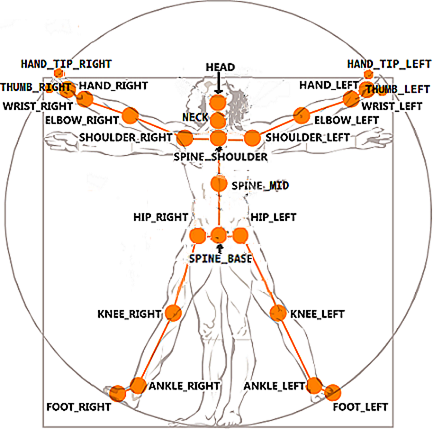
\includegraphics[width=.8\linewidth]{kinect_sk}
	\end{center}
	\caption{Kinect skeletal body configuration.}
	\label{fig:kinect_sk}
\end{figure}



\subsection{Sequential deep learning for ASL}

Here we provide a brief description of various 
deep learning architectures for modeling sequential data and ultimately discuss 
the approaches proposed in this paper for ASL recognition. 
%
Like most  machine learning models,  artificial neural networks (ANN)
learn a mapping function from an input domain to an 
output domain. Usually, the 
input to an ANN is a 1-dimensional 
or multidimensional vector and the 
output is a 1-dimensional 
vector. The training procedure starts 
with initial values for the different 
network parameters that are updated via the 
back propagation algorithm. 
%The input data goes through a non-linear transformation along the network. Using the output vector, one can do some prediction or regression tasks. The parameters of the network are learned by feeding training data to it continuously. On each iteration, first the network predicts labels for training data, then calculates loss using actual labels and finally updates the parameters based on the calculated loss. This iteration process is repeated for a predefined number of times or until a desirable accuracy is acquired on test data. While updating parameters, it starts from the output layer and move backward to the input layer. As it progresses backward, it propagates loss and calculates gradients of errors with respect to the parameters of each layer in a systematic way. Formally this is known as back propagation algorithm and it is the heart of any neural network based machine learning model. 
The general structure of a ANN is 
a feed forward neural network which consists of an input layer, an output layer and one or more intermediate hidden layers.  These class of 
networks have shown 
strong generalization 
performance accuracy and have the ability to capture 
non linear mapping functions to transform the input to the outputs for classification tasks. 


Specifically, the deep learning based 
Convolutional neural network (CNN)  is  a  variant of the 
feed forward neural network that 
has shown human level accuracy for challenging and large-scale 
image classification tasks~\cite{NIPS2012_4824} by modeling the spatial dependencies that exist within an image. Deep 
learning algorithms have also been successful in modeling sequential/temporal 
dependencies that exists when modeling natural language text \cite{DBLP:journals/corr/Graves13,DBLP:journals/corr/SutskeverVL14,DBLP:journals/corr/BahdanauCB14} and spatio-temporal applications \cite{DBLP:journals/corr/abs-0705-2011}. 

%also dependency over time \ie, information at certain point depends on information from a previous point or a future point or both. %One very common example of such data is natural language. Say for example, we want to predict the next word in the blank position of the sentence ``Her mother is a school teacher. $\rule{1cm}{0.15mm}$ teaches in ABC high school''. We can easily see that the blank position is a pronoun which refers to the word \emph{mother} in the previous sentence. But if the word were \emph{father} instead of the word \emph{mother} then the pronoun at the ``$\rule{1cm}{0.15mm}$'' position would be changed too. This example shows an temporal dependency in data.
\begin{figure}[h]
	\begin{center}
		%\fbox{\rule{0pt}{2in} \rule{0.9\linewidth}{0pt}}
		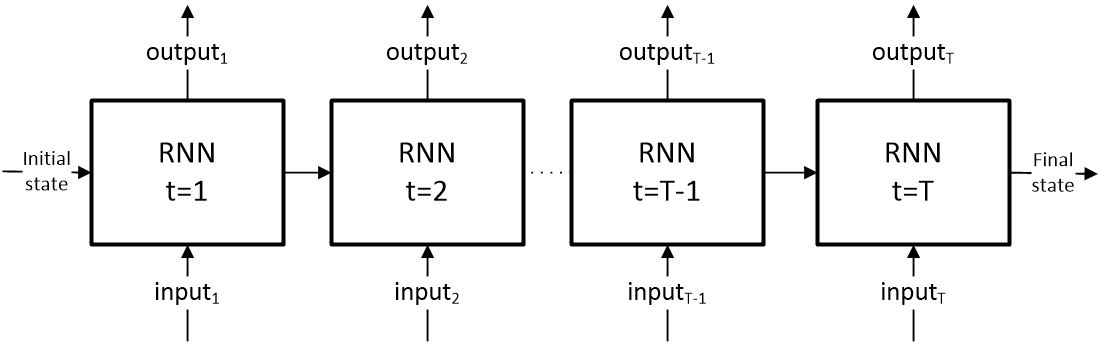
\includegraphics[width=\linewidth]{rnn_network2}
	\end{center}
	\caption{An RNN networks unrolled over T time steps. At each time step the network has one raw input and one processed state input from previous time step. Combining these two it produces embedding for current time step.}
	\label{fig:rnn_network}
\end{figure}
 

%Although feed forward neural networks have shown tremendous accuracy in finding spatial pattern in data, it 
%can not efficiently capture such kind of temporal dependencies. One of main reasons behind this weakness is that 
%it sees the whole input data at once and then it keeps 
%transforming the data through its hidden layers until reaches the 
%final layer. In other words it has to capture the patterns as a whole from the input data. %We can solve this problem if there is a mechanism which first allows us to input a portion of data in an order and then models it. Then it takes as input the second portion of the ordered data, fuses it with modeled output from the first step and then models the fused data. Keep doing this until the final portion of our ordered data will allow us to capture temporal dependencies in our data.

To solve sequential modeling of data, Recurrent neural network (RNN) were 
introduced \cite{DBLP:journals/corr/Lipton15}. RNNs are considered a  variation of ANN and are 
suitable for capturing temporal dynamics within 
data. Figure \ref{fig:rnn_network} shows a high level view of such network. 
Eq~\ref{eq:rnn_eq} shows the equations of such a  RNN. Here $x_t$ is the current input and $h_{t-1}$ is the previous RNN state. $U$ and $V$ are the network parameters associated with $x_t$ and $h_{t-1}$,
respectively. $\phi$ is a non-linear function. Some common choices for this function are \textit{sigmoid}, \textit{ReLu} and \textit{tanh}. 

\begin{equation}
\label{eq:rnn_eq}
\begin{aligned}
g(\mathbf{x_t}, \mathbf{h_{t-1}}) & = U\mathbf{x_t} + V\mathbf{h_{t-1}} \\ f & = \phi(g)
\end{aligned}
\end{equation} 

Two of the most important differences between the 
RNN and feed forward neural networks are time ordered input and network parameter sharing. We can see 
from Figure~\ref{fig:rnn_network} that input is fed to the network in different time steps, not at once like 
the feed forward case. However,
the parameters the network learns throughout different time steps are same. At any time step the network processes the 
current input along with 
previously seen and processed data. This helps to capture the temporal dynamics in data. 


However, this 
basic RNN has problem dealing with long term dependencies in data \cite{DBLP:journals/corr/abs-1211-5063}. This is because the 
basic RNN has no control over what it should learn and what it 
should forget. The approach keeps updating its memory which is not desirable in most practical cases. Sometimes a memory from the 
long past could be useful for current prediction than a memory from the recent past. Another problem which makes training a RNN problematic 
is the  vanishing gradient problem \cite{DBLP:journals/corr/abs-1211-5063}. Since,  network parameters of an RNN are shared over time, at any time step the error derivative not only depends on the current input of network but also on the previous state of the network. The 
multiplicative term of error derivatives back to time step 0 is used 
to calculate error derivative of current time. This is a modification of back propagation algorithm and known as
back propagation through time (BPTT) \cite{58337}. If individual gradients are close to zero this multiplicative term tends towards 
zero and eventually these 
gradients disappear. The opposite can also happen, which is called exploding gradient problem.  However,
this is more obvious and easy to detect. The vanishing gradient problem is not easy to detect and leads to failures. 

Some solutions to above problems involve 
careful initialization of network parameters or  early stopping  \cite{DBLP:journals/corr/abs-1211-5063}. But most effective solution is 
to modify the RNN architecture so that it has a memory state (cell) at every timestep input  that can control what to remember and what to forget. This architecture is referred by the 
long short term memory (LSTM) network \cite{Hochreiter:1997:LSM:1246443.1246450}. Another similar architecture called gated recurrent unit (GRU) has been also proposed and shown to be robust
against the 
vanishing/exploding gradient problem \cite{DBLP:journals/corr/ChoMGBSB14}.

\subsection{Long short term memory} \label{lstm_sec}
As we see from Eq~\ref{eq:rnn_eq}, at each time step, traditional RNN can be 
seen as a nonlinear function of the current input and the previous step. While vanilla RNN is a 
direct transformation from the previous state and the current input, the 
LSTM takes a different approach. It maintains an internal memory and  has a 
mechanism to update and use that memory. The mechanism consists of four separate neural networks also 
called gates. Figure~\ref{fig:lstm_cell} shows a cell of an LSTM network.
%\begin{figure}[h]
%	\begin{center}
%		%\fbox{\rule{0pt}{2in} \rule{0.9\linewidth}{0pt}}
%		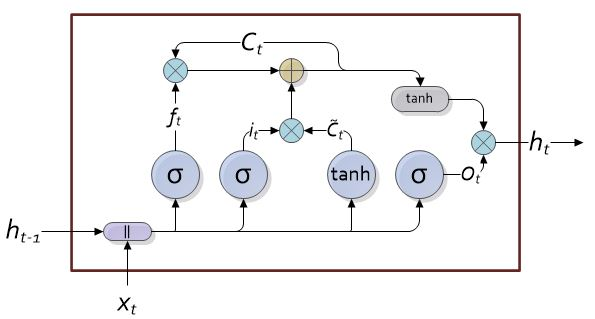
\includegraphics[width=\linewidth]{lstm_cell}
%	\end{center}
%	\caption{An LSTM cell}
%	\label{fig:lstm_cell}
%\end{figure}
Forget, input, update and output gates are represented by four circles and symbolized as $f_t$, $i_t$, $\tilde{C_t}$ and $o_t$, respectively. $\oplus$ and $\otimes$ represents element wise addition and multiplication, 
respectively. $*$ represents matrix multiplication. Two vertical bars inside the rounded rectangle means the 
concatenation operation on its inputs. 
\begin{equation}
\label{eq:lstm_eq}
	\begin{aligned}
		\mathbf{h_t} &= \mathbf{o_t} \otimes tanh(\mathbf{C_t}) \\
		\mathbf{o_t} &= \sigma(W_o * concat(\mathbf{h_{t-1}}, \mathbf{x_t})) \\
		\mathbf{C_t} &= (\mathbf{f_t} \otimes \mathbf{C_{t-1}}) \oplus (\mathbf{i_t} \otimes \mathbf{\tilde{C}_t)}  \\
		\mathbf{i_t} &= \sigma(W_i * concat(\mathbf{h_{t-1}}, \mathbf{x_t})) \\
		\mathbf{\tilde{C}_t} &= tanh(W_{\tilde{C}} * concat(\mathbf{h_{t-1}}, \mathbf{x_t}))
	\end{aligned}
\end{equation}

\begin{figure}[h]
	\begin{center}
		\begin{subfigure}{.45\textwidth}
			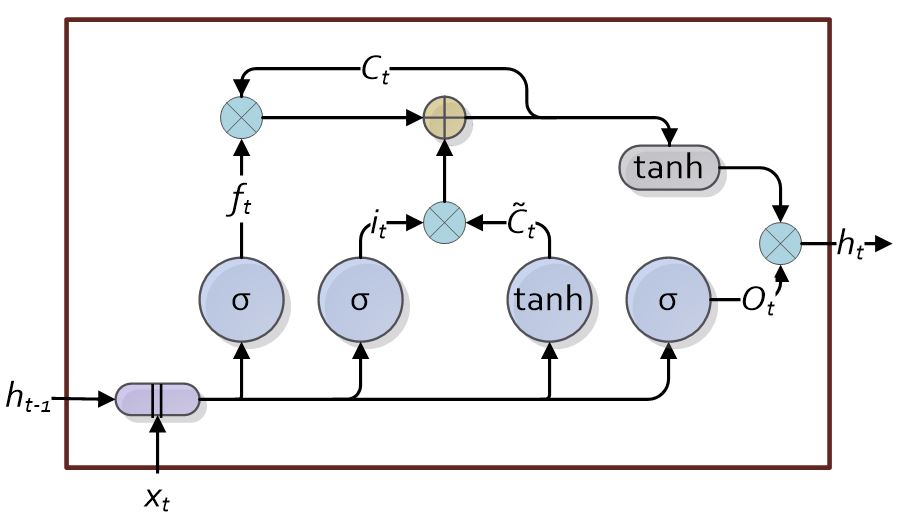
\includegraphics[width=\linewidth, height=.2\textheight]{lstm_cell3}
			\caption{}
			\label{fig:lstm_cell} 
		\end{subfigure}
		
		\begin{subfigure}{.45\textwidth}
			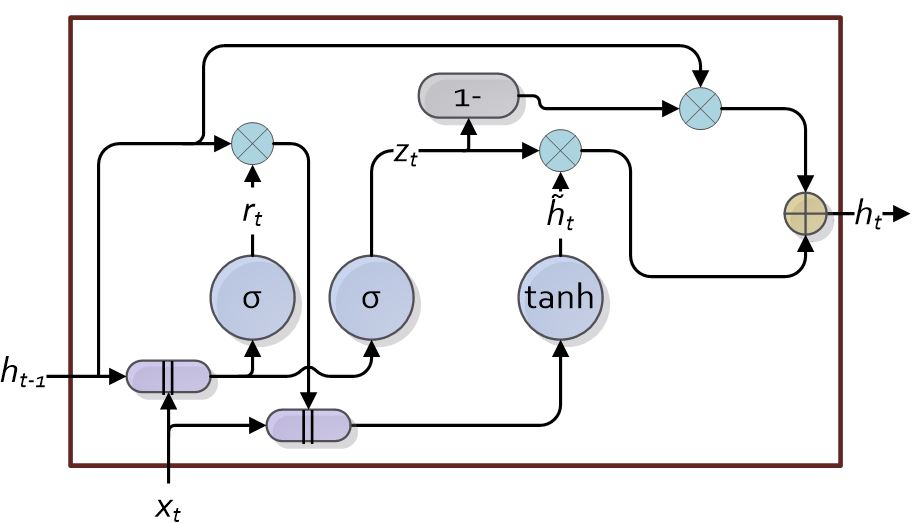
\includegraphics[width=\linewidth, height=.2\textheight]{gru_cell3}
			\caption{}
			\label{fig:gru_cell} 
		\end{subfigure}
	\end{center}
	\caption{a) an LSTM, b) a GRU cell.}
	\label{fig:lstm_gru_cells}
\end{figure}

Figure~\ref{fig:lstm_cell} shows input at the current time step $x_t$ and the 
previous state $h_{t-1}$ enter into the cell and get concatenated. Then the forget gate processes it to remove
unnecessary information and outputs $f_t$ which gets multiplied with the previously 
stored memory $C_t$ and produces a refined memory for the current time. Meanwhile, the input 
and  update gate process the concatenated input and convert it into a candidate memory for the current time step. The refined memory from the previous step and proposed candidate memory of the current step get added to produce the final memory for the current step. This addition could render the output out of scale. Because of that, a squashing function (hyperbolic $tan$) is used 
in our case. This scales the elements of the output vector into a fix range. Finally $o_t$, the output 
from output gate gets multiplied with output from the squashing function and produces the output for the current time step. Eq~\ref{eq:lstm_eq} shows the equations of LSTM where $concat(\mathbf{x},\mathbf{y})$ is 
concatenation of input vectors $\mathbf{x}$ and $\mathbf{y}$.

\begin{figure*}
	\begin{center}
		%		\fbox{\rule{0pt}{2in} \rule{.9\linewidth}{0pt}}
		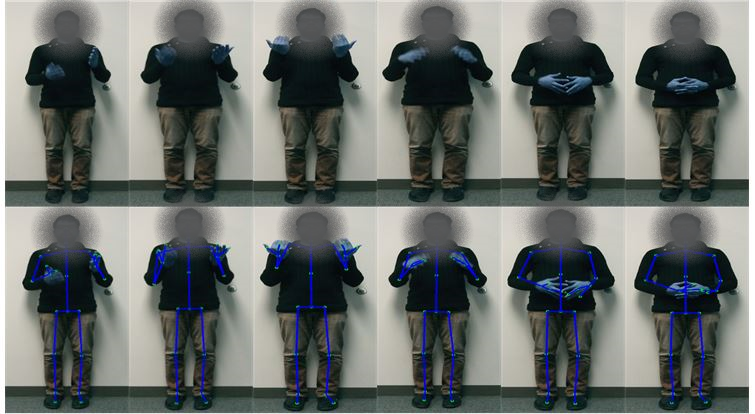
\includegraphics[width=.8\linewidth]{ac_person1_faceoff}
	\end{center}
	\caption{Example of a sign (Air Condition) performed by a person. Top row shows six frames from RGB videos increasing in time from left to right. Bottom row shows exactly same frames but with skeleton data visualization on it. Subject's face is intentionally made unrecognizable.}
	\label{fig:ac_person1}
\end{figure*}

\subsection{Gated recurrent unit}
A gated recurrent unit (GRU) is another variation of RNN for modeling temporal dynamics of data. It works in the same way as LSTM
but has a simpler construction. Like LSTM it has the mechanism to control flow of information over time but it lacks the separate memory cell. 
Figure~\ref{fig:gru_cell} shows an example of GRU cell. Symbols represent similar things as described in subsection~\ref{lstm_sec}. 
%\begin{figure}[h]
%	\begin{center}
%		%\fbox{\rule{0pt}{2in} \rule{0.9\linewidth}{0pt}}
%		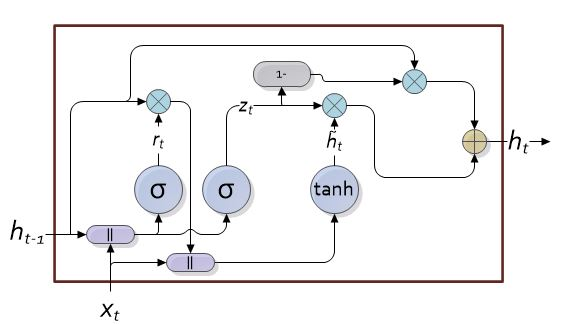
\includegraphics[width=\linewidth]{gru_cell}
%	\end{center}
%	\caption{A GRU cell}
%	\label{fig:gru_cell}
%\end{figure}
To better understand GRU cell, first we have to look at the output of it. The output is formed by a weighted linear sum of two components $\tilde{h}_t$ and $h_{t-1}$ as seen from the Eq.~\ref{eq:gru_eq}. 
%Here $concat(x,y)$ means concatenation of input vectors $x$ and $y$. Element wise multiplication and addition are represented by $\otimes$ and $\oplus$ respectively.
\begin{equation}
	\label{eq:gru_eq}
	\begin{aligned}
		\mathbf{h_t} & = (1-\mathbf{z_{t}})\mathbf{h_{t-1}} \oplus \mathbf{z_{t}}\mathbf{\tilde{h}_t} \\
		\mathbf{z_{t}} &= \sigma(W_z*concat(\mathbf{h_{t-1}}, \mathbf{x_t})) \\
		\mathbf{\tilde{h}_t} &= tanh(W_{\tilde{h}}*concat(\mathbf{r_t} \otimes \mathbf{h_{t-1}}, \mathbf{x_t})) \\
		\mathbf{r_t} &= \sigma(W_r*concat(\mathbf{h_{t-1}}, \mathbf{x_t})) \\
	\end{aligned}
\end{equation}
$\tilde{h}_t$ represents the 
newly proposed candidate embedding and $h_{t-1}$ is simply the previous state. Candidate embedding $\tilde{h}_t$ is a function of the current input and purified previous state. This purification is achieved by the reset gate $r_{t}$, which decides
what portion of the 
previous state should contribute to the 
candidate embedding $\tilde{h}_t$. Reset gate $r_{t}$ itself is a separate neural network and its output close to 0 means network takes a small portion of previous state to form a current candidate state embedding. The update gate $z_{t}$ decides what fractions of the candidate state and the previous state comprise the new state. It does so by taking a weighted some of the candidate state and the previous state. The weights are $z_{t}$ and $1-z_{t}$. %This whole new state is outputted where in case of LSTM, the output of the new state is controlled by an output gate as shown in Eq. ~\ref{eq:lstm_eq}.  


\subsection{Our approach}
ASL signs are usually performed using two hands, head movements and in several  
cases facial expressions. 
%{\bf AL-provide examples of signs that show facial expressions. see our proposal}. 
Motion dynamics of 
two hands are responsible for creating different cues for various signs. Each joint in two hands and face area follows a specific sequential pattern for a particular gesture sign. For example, from Figure~\ref{fig:ac_person1} we see that 
the person is performing gesture for \textit{air condition}. We can see that, for this sign first, one has to lift and show palm area of the left hand and then he/she has to lift both hands and make a back and forth motion with all fingers. This is basically a sequence of joints in both hands. We propose to use the LSTM and GRU based models for modeling these 
sequential dependencies for distinguishing between different ASL signs. 

We notice that the joints located above the waist are mostly useful in case of sign language. Hence, we take only 12 joints into
consideration for  our experiments. These joints come from both hands, head, neck and spine area. Figure~\ref{fig:rnn_impl} shows our implementation. For each time step, first, we concatenate 3D coordinates of 12 joints and then feed to our RNN network. Finally, we take the final state of the network and feed 
it to a softmax layer to 
get prediction probabilities over our classes.

\begin{figure*}[h]
	\begin{center}
		%\fbox{\rule{0pt}{2in} \rule{0.9\linewidth}{0pt}}
		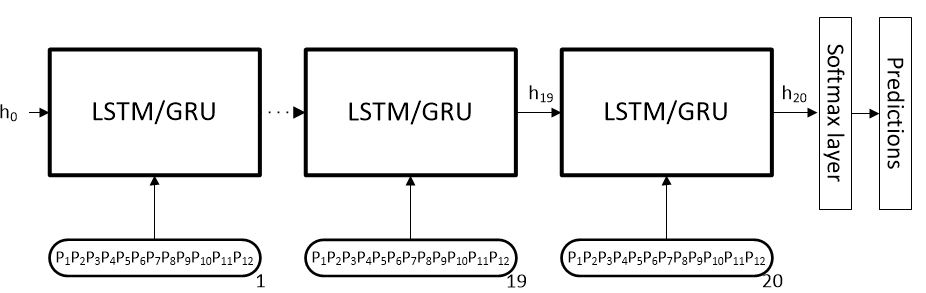
\includegraphics[width=.8\linewidth]{rnn_impl}
	\end{center}
	%	\caption{Implementaion of RNN models x, y, z}
	\caption{Implementation of RNN models to recognize ASL from skeletal data. Input at each time step is a concatenation of 3D coordinates of 12 joints denoted by rounded corner input boxes above. $P_i$ is the $(x, y, z)$ of $i^{th}$ joint. Subscript of each input vector represents time step. We used 20 time steps for each sample data in our experiments as shown above.}
	\label{fig:rnn_impl}
\end{figure*}


\section{Experiments}
In this section, we provide an overview of the proposed experiments along with a protocol of dataset collection. 
We are also going to describe a calibration mechanism we propose, to find a good seed
percentage of train data for a test person. Then we are going to present implementation details and results we got from experiments. 

\subsection{Data collection protocol}

Since no skeletal dataset was publicly available for
ASL, the first goal of this project is to build our own 
database of ASL signers. The database is publicly available \footnote{Email author for dataset and codes}.

%{\bf Al-Amin add a link to the dataset}
%%
%{\bf Al-Amin add in the intro. that dataset is a contribution for this work}


Specifically, we collected  ASL samples 
for 4 signers performing 
  6 daily activities related signs with each ``sign'' repeated 20 times. This resulted in a total of 480 samples 
  across the four participants. Motivated by our overall objective to develop
  accessible technologies for deaf and hard of hearing persons, we chose 
  six activities that were considered as important in their daily life. Table \ref{table:asl_signs} 
  shows these six ASL signs. We used the Kinect v2.0 for the data collection. For each participant 
the sensor was placed at different distances from the participant for the 
different repetitions. This was done to simulate the real world scenarion of having the external sensor 
at different distances from the end user. 

Figure~\ref{fig:ac_person1} shows an examplar data. It shows six frames from the signing of 
\textit{air conditioning} at the top with 
skeletal joints drawn  to them at the bottom.  The skeleton tracking data for the six signs 
are shown in Figure \ref{fig:sk_dat_viz}.


\begin{table}[h]
	\begin{center}
		\begin{tabular}{|c|c|c}
			\hline
			Wake Up & Turn on Thermostat\\
			\hline
			Interpreter & Air Condition\\
			\hline
			Open Door & Close Door\\
			\hline
		\end{tabular}
	\end{center}
	\caption{Selected ASL signs.}
	\label{table:asl_signs}
\end{table}

\subsection{Preprocessing}
Kinect skeleton sequences are 
captured in camera coordinate system \ie, the 
camera position is considered to be the
the origin. To make sequences invariant to different 
camera positions and body-shapes, we convert sequences 
into body coordinate system. We pick a joint location 
and make it the 
origin and then  subtract $(x, y, z)$ locations of all
other joints from it. Also, different collected samples have
different frame lengths and a video file with frame rate of 32 fps has negligible difference between two consecutive frames. Hence, we sample 
a fix number of frames from each sample. We used this fixed number \textit{T} as  20. 

%{\bf Al - see above XXX}


\subsection{Evaluation protocol}
\label{sec:ev_prot}
Our experiment on the dataset is two fold. First, we did experimentation 
with two deep learning sequence models (GRU, LSTM)  and a dynamic time warping (DTW) based comparative method. Secondly, we proposed a calibration mechanism which essentially can infer what fraction of data from an unseen test subject is needed to boost performance of our models. This calibration experiment is done in cross subject manner \eg, we train our models on some subjects and test on a different subject. This makes a lot of sense in real life situation where a trained model has to perform well on unseen data. 

%{\bf - Al write a detailed subsection on dtw and how it is implementented 00 call that subsection comparative methods.}

%{\bf - the experimental protocol should be about how you train the models and how you benchmark the results}

\subsection{Comparative method}
We used dynamic time warping (DTW) for comparing performance with our RNN methods. It is one of the most used measure of similarity between two sequences. DTW can find optimal global alignment between two sequences. Unlike element wise euclidean distance, it takes temporal distortion into account. For this reason, even if two sequences are similar in shape but in out of phase, DTW will be able to find significant similarity. In skeletal data, each ASL sign is a combination of several body joints, 12 joints in our case. To calculate similarity between two sign, we measure the DTW distance between same joint and sum up these 12 distances to get the total similarity measure.
\begin{figure*}
	\begin{center}
		%\fbox{\rule{0pt}{2in} \rule{0.9\linewidth}{0pt}}
		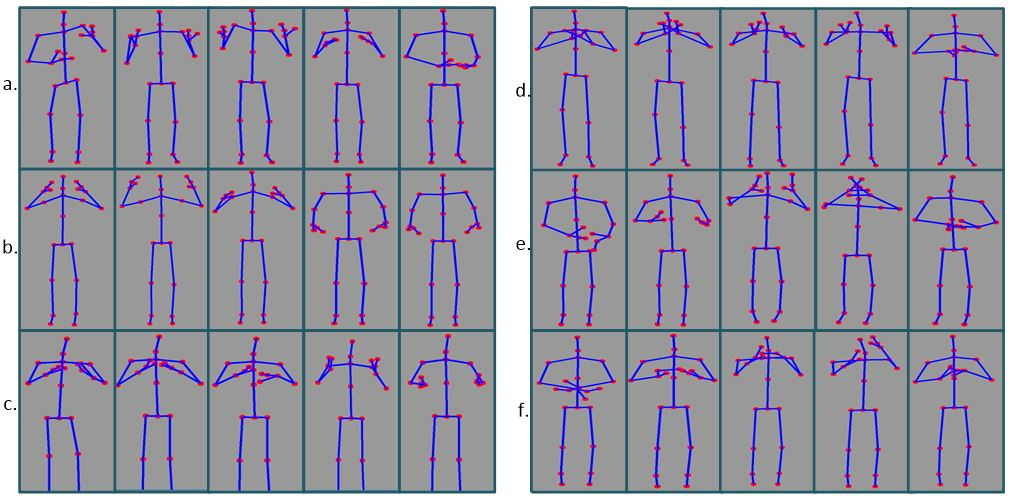
\includegraphics[width=.8\linewidth]{sk_data_viz}
	\end{center}
	%	\caption{Implementaion of RNN models x, y, z}
	\caption{Skeleton visualization of classes in the dataset -- a. Air condition, b. Wake up, c. Interpreter, d. Door open, e. Door close, f. Thermostat on.}
	\label{fig:sk_dat_viz}
\end{figure*}


\begin{table}[h]
	\begin{center}
		\begin{tabular}{|m{1cm}|m{5cm}|}
			\hline
			Terms & Description\\
			\hline\hline
			$D_{train}$ & Training data, whole data from the subjects other than the test subject \\
			\hline
			$D_{test}$ & Test data, $50\%$ data from test subject used for testing models\\
			\hline
			$D_{seed}$ & Seed data, $50\%$ data from test subject used for boosting up model's performance on $D_{test}$\\
			\hline
		\end{tabular}
	\end{center}
	\caption{Different terminologies regarding data split for one test subject.}
	\label{table:terminology_eval}
\end{table}

Table \ref{table:terminology_eval} represents some terminologies helpful to understand calibration mechanism described next.
We have data on four different subjects. First, we choose a test subject and take out $50\%$ of data from this subject as test data say $D_{test}$. We use other $50\%$ of data as seed data say, $D_{seed}$ to train model along with the data from other three subjects say, $D_{train}$. We first train the model only with $D_{train}$ and test on $D_{test}$. Then we train our model with $D_{train}$ and $10\%$ from $D_{seed}$ and again test on $D_{test}$. Then again we train the model with $D_{train}$ and this time $20\%$ of $D_{seed}$ and test on $D_{test}$. As we increase the seed data in our training data, we should expect better test accuracy. We keep doing this until we use up to full $D_{seed}$ for training with $D_{train}$ and record different testing results on $D_{test}$. We repeat the whole procedure by taking each subject as a test subject one at a time. We want to see here what fraction of seed data is required during training to get a good performance from our model. Figure~\ref{fig:train_test_dat} shows data splitting strategy for better understanding.

\subsection{Parameter selection}

We used same value for hyper-parameters such as learning rate, state size of RNNs and batch size  for both the LSTM models. We performed 
a grid search for finding best hyper-parameters. Our experiments found the best learning rate as $5e^{-4}$ and the state size for RNNs as 60. For each joint, the state size is 5 which gives us the total 
state size of 60 for 12 joints. We used Adam Optimizer for optimizing our networks~\cite{DBLP:journals/corr/KingmaB14}. We used this 
optimizer because it has shown superior performance in training different types of network. It also adapts learning rate and 
decay rate as training continues. We used mini-batch size of 1 which means the network updates it's parameter after seeing one training example. We keep training our network until a good accuracy is achieved on the test set.
%a {\bf XXX CHECK validation set}. 
\begin{figure}[h]
	\begin{center}
		%\fbox{\rule{0pt}{2in} \rule{0.9\linewidth}{0pt}}
		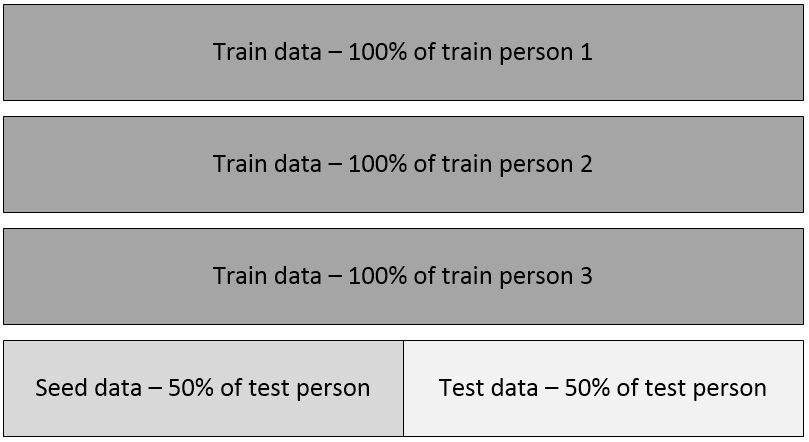
\includegraphics[width=\linewidth, height=.2\textheight]{train_test_dat}
	\end{center}
	\caption{Train and test data split for a test person.}
	\label{fig:train_test_dat}
\end{figure}
To avoid over-fitting of the network we follow the 
early stopping strategy. If there is no increase in the test accuracy for 15 epochs  we  stop training. 

\subsection{Implementation details}

We implemented our models using TensorFlow deep learning library 
version $1.7$ \footnote{https://www.tensorflow.org/}. These experiments were run on ARGO, a research computing 
cluster provided by the Office of Research Computing at 
George Mason University, VA \footnote{URL:http://orc.gmu.edu}.
All RNN jobs were run on a GPU cluster node which has four tesla K80 gpu and DTW jobs were run on an ordinary cluster node with multiple CPUs.
%{\bf Describe Argo nodes in 2 lines and say all run times were reported on that machine configuration}


\section{Results}

Table \ref{table:result_table} shows the classification 
performance of the LSTM and GRU in comparison to the baseline DTW-based approach. We follow the experimental protocol as described in 
Section \ref{sec:ev_prot} where 0\% seed data indicates cross-subject performance where no training data from the subject (person) in test is used during the training phase. 
We observe that, with no or less seed $(<=10\%)$ the LSTM/GRU models outperform the DTW by $10\%-25\%$ on average across the four subjects. As we increase the amount of seed data from the person 
under test set we see that with 30\% of data yields high classification performance results. For DTW approach, the 
 accuracy is relatively lower with 0\% seed. But, with small amount of seed ($20\%-30\%$), it reaches accuracy in the range of $95-96\%$. 
% DTW compares the distances of one sample of test set with every other sample in training set and with little introduction of data from same class and subject (seed) would always give minimum distance between test sample and seed. Table~\ref{table:result_table} shows the results for each combination of a test person, a \% of seed data used in training for that person and a network type.
 
 
 %{\bf Al Amin - why is the DTW result 54\% in 10\%}
 
\begin{table}[h]
	\begin{center}
		\begin{tabular}{|m{1em} | m{3em} | m{1.5em} | m{1.5em} | m{1.5em} |m{1.5em} |m{1.5em} |m{1.5em} |}
			\hline
			%			 & \multicolumn{6}{c}{\% of training data} \vline\\
			%			\hline
			& \% seed & $0\%$ & $10\%$ & $20\%$ & $30\%$ & $40\%$ & $50\%$\\
			\hline
			\multirow{3}{3.5em}{$P_1$}
			& DTW & $0.66$ & $0.89$ & $0.95$ & $0.96$ & $0.96$ & $0.96$\\
			\cline{2-8}
			& LSTM & $0.82$ & $\textbf{1.00}$ & $0.97$ & $\textbf{0.98}$ & $\textbf{1.00}$ & $\textbf{1.00}$\\			
			\cline{2-8}
			& GRU & $0.85$ & $0.96$ & $0.95$ & $0.97$ & $\textbf{0.98}$ & $\textbf{1.00}$\\
			\hline
			\multirow{3}{3.5em}{$P_2$}
			& DTW & $0.85$ & $0.89$ & $0.90$ & $0.91$ & $0.94$ & $0.95$\\
			\cline{2-8}
			& LSTM & $0.90$ & $0.93$ & $\textbf{0.98}$ & $0.93$ & $0.93$ & $\textbf{0.98}$\\
			\cline{2-8}
			& GRU & $0.88$ & $0.93$ & $0.91$ & $0.92$ & $\textbf{0.98}$ & $0.95$\\
			\hline
			\multirow{3}{3.5em}{$P_3$}
			& DTW & $0.50$ & $0.54$ & $0.82$ & $0.94$ & $0.96$ & $0.96$\\
			\cline{2-8}
			& LSTM & $0.68$ & $0.65$ & $0.68$ & $0.75$ & $0.82$ & $\textbf{0.93}$\\
			\cline{2-8}
			& GRU & $0.65$ & $0.72$ & $0.68$ & $0.79$ & $0.80$ & $0.86$\\
			\hline
			\multirow{3}{3.5em}{$P_4$}
			& DTW & $0.69$ & $0.82$ & $0.89$ & $0.93$ & $0.94$ & $0.95$\\
			\cline{2-8}
			& LSTM & $0.89$ & $0.93$ & $0.93$ & $0.93$ & $0.93$ & $\textbf{0.96}$\\
			\cline{2-8}
			& GRU & $0.91$ & $0.93$ & $0.93$ & $0.93$ & $0.91$ & $\textbf{0.94}$\\
			\hline
			\multirow{3}{3.5em}{$\bar{P}$}
			& DTW & $0.69$ & $0.81$ & $0.90$ & $0.93$ & $0.94$ & $0.96$\\
			\cline{2-8}
			& LSTM & $0.83$ & $0.88$ & $0.90$ & $0.90$ & $0.92$ & $\textbf{0.97}$\\
			\cline{2-8}
			& GRU & $0.82$ & $0.88$ & $0.87$ & $0.90$ & $0.92$ & $0.94$\\
			\hline
		\end{tabular}
	\end{center}
	\caption{Classification performance across four subjects  $P_i$ denotes the $i^{th}$ subject and $\bar{P}$ denotes the average accuracy of all subjects.}
	\label{table:result_table}
\end{table}

\begin{figure}
	\begin{center}
		\begin{subfigure}{.45\textwidth}
			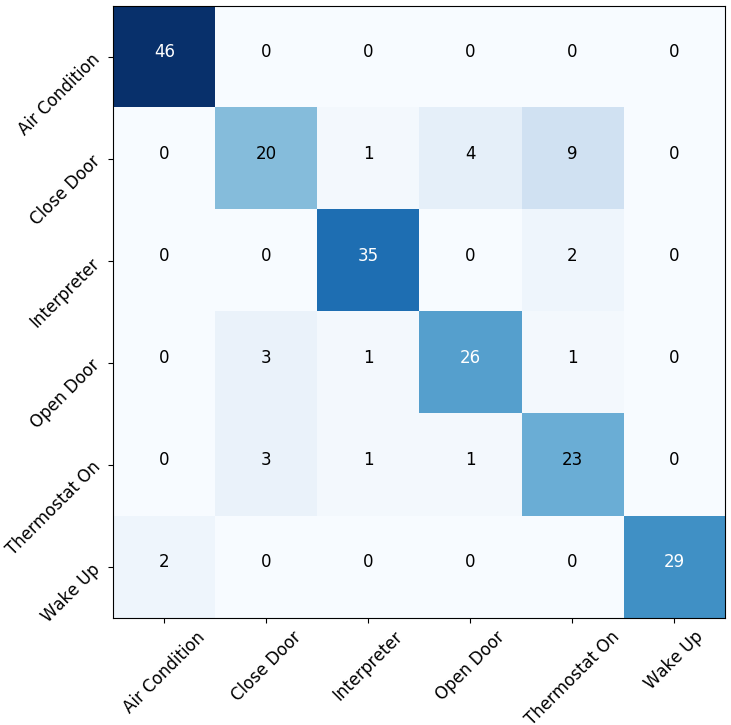
\includegraphics[width=\linewidth, height=.25\textheight]{cm_zero_percent_cropped}
			\caption{}
			\label{fig:cm_zero} 
		\end{subfigure}
		
		\begin{subfigure}{.45\textwidth}
			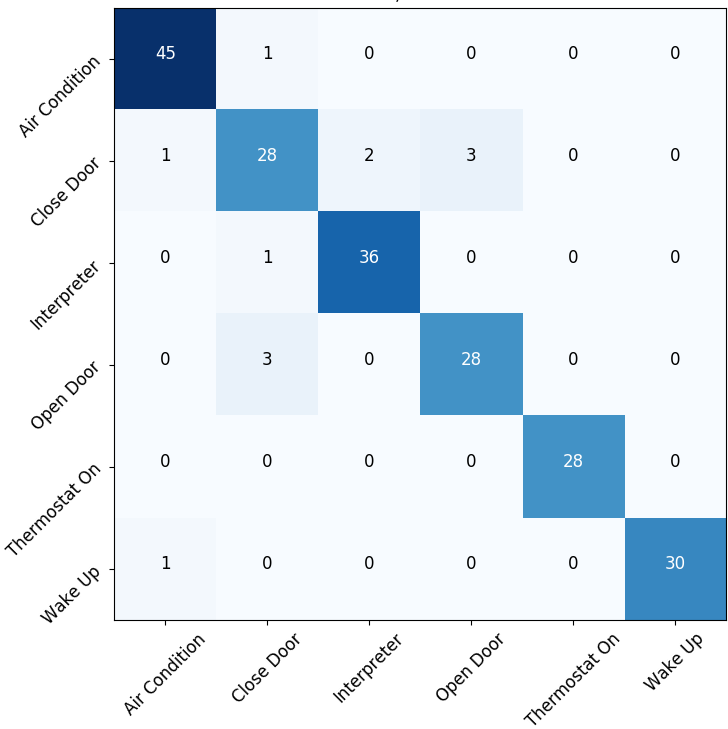
\includegraphics[width=\linewidth, height=.25\textheight]{cm_thirty_percent_cropped}
			\caption{}
			\label{fig:cm_thirty} 
		\end{subfigure}
	\end{center}
	\caption{Confusion matrix for $0\%$ (a) and $30\%$ (b) seed data for LSTM model}
	\label{fig:conf_mat}
\end{figure}


\begin{table}[h]
	\begin{center}
		\begin{tabular}{|c|c|c|}
			\hline
			Model type & Mean accuracy & Std. deviation\\
			\hline\hline
			LSTM & $\textbf{0.95}$ & $0.03$\\
			\hline
			GRU & $0.94$ & $0.02$ \\
			\hline
		\end{tabular}
	\end{center}
	\caption{Statistics of results from 5-fold cross validation.}
	\label{table:result_conv}
\end{table}
%\begin{figure*}
%	\begin{center}
%		\begin{subfigure}{.8\textwidth}
%			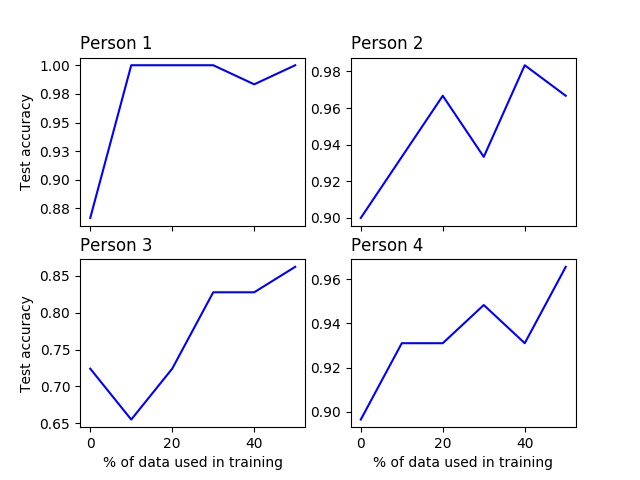
\includegraphics[width=\linewidth, height=.3\textheight]{result_lstm}
%			\caption{}
%			\label{fig:result_lstm} 
%		\end{subfigure}
%		
%		\begin{subfigure}{.8\textwidth}
%			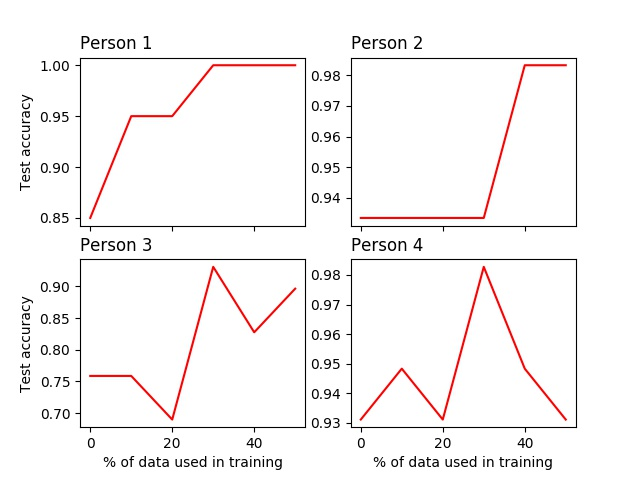
\includegraphics[width=\linewidth, height=.3\textheight]{result_gru}
%			\caption{}
%			\label{fig:result_gru} 
%		\end{subfigure}
%	\end{center}
%	\caption{Test accuracy. X-axis represents percentage of data from the test subject used in training and Y-axis is the test accuracy on $50\%$ hold out data for test subject. (a) Test accuracy for LSTM network. Each plot represents accuracy on test data for each subject in our dataset. (b) Test accuracy for GRU network in same way as (a).}
%	\label{fig:result_comp}
%\end{figure*}
We observe from the result that, for RNN methods the highest accuracy is obtained using 30\% or more seed data. This suggests that, even if we have a small amount of seed data for a test persons, our system can boost up to a higher accuracy quickly which is important for practical system. 
%In a practical scenario, system will be able to recognize new subjects correctly within a short period of subject's interaction with the system. 
Although DTW achieve comparable results in some cases, runtime increases rapidly as training sample increases. In our case, DTW takes 2.5 hours to complete, while, training RNNs requires 1.11 hours on average.
%{\bf Al Amin do you have a TABLE on time}
%Figure~\ref{fig:result_comp} shows plots of test accuracy vs percentage of data used in training. It shows the LSTM results at the top and the GRU results at the bottom. Plots are also suggesting that $30\%$ or more of seed data is good enough for a performance increase to the model. We also analyzed confusion matrix to see what classes confuses each other and found that increasing percentage of seed data in training decreases confusion. 

Figure~\ref{fig:cm_zero} shows the 
 confusion matrix  across the six classes when no seed data is used in training for LSTM model. We can see that for the 
 sign ``Close Door'' is confused with the sign ``Thermostat On'' and ``Open Door''. However, in Figure~\ref{fig:cm_thirty} we observe that, with only increase of seed data to 30\% in training  reduces these mis-predictions significantly. We can see from skeleton visualization in Figure~\ref{fig:sk_dat_viz} that the signs for ``Open Door''
 ``Close Door'' and ``Thermostat On'' are  similar with regards to the joint movements. 
 
 
We also tested our model in a  conventional train test split manner. 
%In that case, we took $30\%$ of whole data as test data. Table~\ref{table:result_conv} shows accuracy for both type of RNN models after performing k-fold cross validation 
%{\bf Al Amin is it k-fold or test/train split}. 
We did five-fold cross validation in this case. Table~\ref{table:result_conv} shows statistics across five runs of cross validation. We observe that, LSTM works little better than GRU.
We did not perform DTW in this experiment since the pairwise computation is time consuming. Further, the scope of  this work is to initiate sequence modeling using deep learning architectures for ASL recognition.

 
\section{Conclusion}
A multi-modal dataset for ASL recognition is introduced. Dataset consists of total 480 samples related to six daily activities of deaf or hard-of-hearing people. A cross subject evaluation technique is shown and experimental result shows high testing accuracy. Our proposed calibration mechanism shows what percentage of training data is required from a subject to boost performance. Although, the margin of the dataset is not large, our result suggests a promising direction towards sign language recognition research. Implemented methods show effectiveness of sequential models (RNNs) in practical problem solving. Our future plan is to build a large scale benchmark dataset for ASL recognition by augmenting the current dataset and develop machine learning models that can recognize sentence level ASL.


%All text must be in a two-column format. The total allowable width of the
%text area is $6\frac78$ inches (17.5 cm) wide by $8\frac78$ inches (22.54
%cm) high. Columns are to be $3\frac14$ inches (8.25 cm) wide, with a
%$\frac{5}{16}$ inch (0.8 cm) space between them. The main title (on the
%first page) should begin 1.0 inch (2.54 cm) from the top edge of the
%page. The second and following pages should begin 1.0 inch (2.54 cm) from
%the top edge. On all pages, the bottom margin should be 1-1/8 inches (2.86
%cm) from the bottom edge of the page for $8.5 \times 11$-inch paper; for A4
%paper, approximately 1-5/8 inches (4.13 cm) from the bottom edge of the
%page.

%-------------------------------------------------------------------------

{\small
\bibliographystyle{ieee}
\bibliography{egbib}
}


\end{document}
